\documentclass[a4paper,11pt]{article}

\usepackage[english]{babel} 
\usepackage[utf8]{inputenc}
\usepackage[cyr]{aeguill}
\usepackage{stmaryrd}

\usepackage{lmodern} %Type1-font for non-english texts and characters
\usepackage{caption}
\usepackage{subcaption}

\usepackage{graphicx}
\usepackage{hyperref}

\usepackage{epstopdf}


%\hypersetup{	
%colorlinks=true,   %colorise les liens 
%breaklinks=true,  %permet le retour à la ligne dans les liens trop longs 
%urlcolor= blue,    %couleur des hyperliens 
%linkcolor= black, %couleur des liens internes 
%citecolor=black,	 %couleur des références 
%pdftitle={Compte rendu \emph{Traitement numérique du signal}, %informations apparaissant dans 
%pdfauthor={Mélisande Zonta}, %les informations du document 
%pdfsubject={Projet TNS2}	%sous Acrobat. 
%} 

%% Math Packages 
\usepackage{amsmath}
\usepackage{amsthm}
\usepackage{amsfonts}
\usepackage{amssymb}
\usepackage{mathrsfs}
\usepackage{pst-all}
\usepackage{lscape}
\usepackage{pdfpages}
\usepackage{mathabx}


\usepackage{color, colortbl}
\definecolor{lightgray}{gray}{0.85}
\usepackage{multirow}
\usepackage[Algorithme]{algorithm}
\usepackage[noend]{algpseudocode}
\usepackage{tikz}

%\renewcommand{\algorithmicdo}{\textbf{faire}}
%\renewcommand{\algorithmicwhile}{\textbf{tant que}}


\usepackage{a4wide} %%Smaller margins = more text per page.
\usepackage{fancyhdr} %%Fancy headings

\setcounter{secnumdepth}{5}
\setcounter{tocdepth}{5}


\DeclareMathOperator*{\argmax}{arg\,max}
\DeclareMathOperator*{\argmin}{arg\,min}
\graphicspath{{/Users/melisandezonta/Documents/Documents/GTL_courses_second_semester/Computer-Vision/PS1-all/PS1-images/}}

\begin{document}

%\pagestyle{fancy}

\begin{titlepage}
\vspace*{\stretch{1}}

\begin{center}

\includegraphics[scale=0.4]{GT_logo.jpeg}
\end{center}
\vspace*{\stretch{1}}
\hrulefill
\begin{center}\bfseries\huge
   Computer Vision \\
   CS 6476 , Spring 2018\\
   \end{center}
  \begin{center}\bfseries\large
     PS 1\\
    \hrulefill
\end{center}
%\hfill
\vspace*{1cm}
\begin{minipage}[t]{0.6\textwidth}
  \begin{flushleft} \large
    \emph{Professor : }\\
    Cedric Pradalier \\
  \end{flushleft}
\end{minipage}
\begin{minipage}[t]{0.3\textwidth}
  \begin{flushright} \large
    \emph{Author :} \\
    Melisande Zonta \\
  \end{flushright}
\end{minipage}
\vspace*{\stretch{2}}
\begin{flushright}
       \today 
\end{flushright} 
\end{titlepage}

\tableofcontents
\clearpage

\section{Creation of the edges image}



 \begin{figure}[H]
\begin{center}
\begin{tabular}{cc}
	
\includegraphics[width=.5\textwidth]{ps1-1-a-original.png}&
	
\includegraphics[width=.5\textwidth]{ps1-1-a-edges.png}\\
	a&b
\end{tabular}
\end{center}
\caption{ 
\textit{a}. ps1-1-a : Original Image. \textit{b}. ps1-1-a : Edges Image.}
\label{ps1-1-a}
\end{figure}

The Figure 1 is the result of the Canny edge detector to perform the original edge detection.

\section{Hough Method applied on the lines}

 \begin{figure}[H]
\begin{center}
\begin{tabular}{cc}
	
\includegraphics[height=.3\textwidth]{ps1-1-a-original.png}&
	
\includegraphics[height=.3\textwidth]{ps1-2-edges.png}\\
	a&b\\
	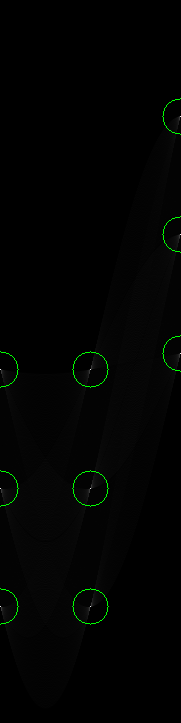
\includegraphics[height=.4\textwidth]{ps1-2-accu-circled.png}&
	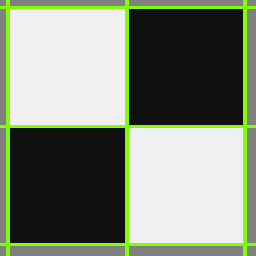
\includegraphics[height=.3\textwidth]{ps1-2-lines.png}\\
	c&d\\
\end{tabular}
\end{center}
\caption{ 
\textit{a}. ps1-2-original : Original Image.  \textit{b}. ps1-2-edges : Edges Image. \\
\textit{c}. ps1-2-accumulator : Hough accumulator array image. \textit{d}. ps1-2-lines : Intensity Image with lines drawn on them.}
\label{ps1-2}
\end{figure}

The Figure 2-c is the result of the voting in the accumulator and the figure 2-d is the associated image with the detected lines. 
In order to get the finest detection possible, a choice was made on the bins size.

Concerning $\theta$  the length of the bin is $$\frac{180}{grid_{size}} + 1$$.
Concerning $d$, the range for values varies from $-d_{max}$ to ${d_{max}}$ with $$d_max = \sqrt{m^2+n^2}$$, $m$ the number of rows of the image and $n$ the number of columns. Hence the length of the bin is $2 \times d_{max}+1$.

The image being a 256px square, the maximum value of d is the diagonal, around 362. Thus the choices we made for the bin result in a rectangular accumulator.

\section{Noise effect on the lines detection}


\subsection{First Step : Smoothing}

\begin{figure}[H]
\centering
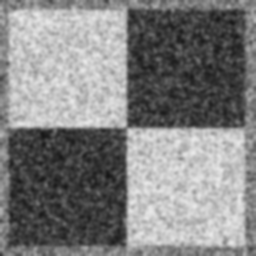
\includegraphics[height = .4\textwidth]{ps1-3-a-image-noisy-smoothed.png}
 \caption{ps1-3-a : Image noisy smoothed }
\label{ps1-3-a}
\end{figure}


The smoothed version using a Gaussian kernel is visible in Figure 3.


\subsection{Second Step : Edges detection}


 \begin{figure}[H]
\begin{center}
\begin{tabular}{cc}

\includegraphics[height  = .4\textwidth]{ps1-3-b-edges.png}&
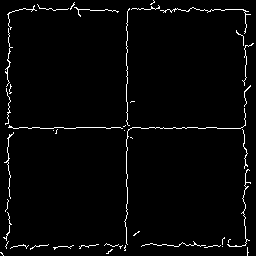
\includegraphics[height = .4\textwidth]{ps1-3-b-edges-image-noisy.png}\\
	a&b
\end{tabular}
\end{center}
 \caption{\textit{a}. ps1-3-b-original : Edges Original Image.  \textit{b}. ps1-3-b-noisy : Edges Smoothed Image. }
\label{ps1-3-b}
\end{figure}

The figure 4.a show the edges resulting from the Canny edge detector on the original image. The figure 4.b show the edges detected on the noisy image.

\subsection{Third Step : Hough Algorithm for lines}

 \begin{figure}[H]
\begin{center}
\begin{tabular}{cc}
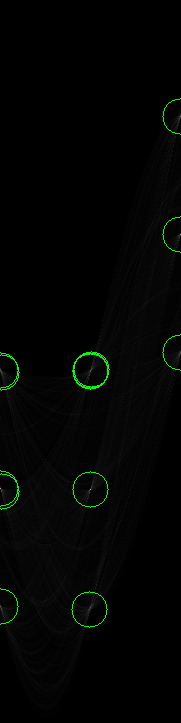
\includegraphics[height = .5\textwidth]{ps1-3-c-accu-circled.png}&
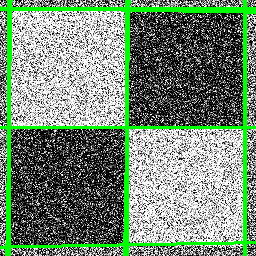
\includegraphics[height = .5\textwidth]{ps1-3-c-lines.png}\\
	a&b
\end{tabular}
\end{center}
 \caption{
\textit{a}. ps1-3-c-accumulator : Hough accumulator array image.  \textit{b}. ps1-3-c-lines : Intensity Image with lines drawn on them. }
\label{ps1-3-c}
\end{figure}

In order to get a good result on the noisy image, we first had to get an image smoothed with a sigma of a few pixels meaning we first had to convolve the image with a standard Gaussian kernel.

Afterwards, we used the Canny edge detector in order to get a relatively good quality of edges, meaning getting each of the 9 edges as in the previous part.

I finally used the Hough line detection method to extract the 6 edges, which required lowering the threshold to get all of them. We see on Figure 5.b that vertical edges are represented by multiple lines instead of a single one. This is due to the fact that peaks on the edge of the theta axis get wrapped around the matrix and detected twice). This results in several lines with a little difference in angle.

\section{Lines detection on a more complicated image}

\subsection{First Step : Smoothing}

\begin{figure}[H]
\centering
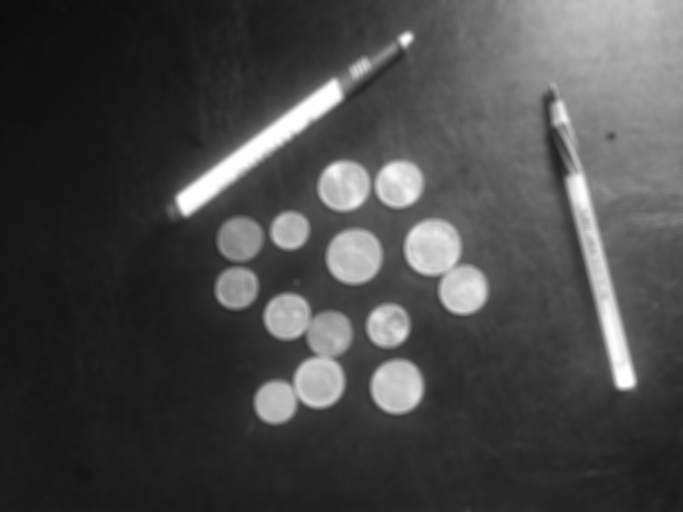
\includegraphics[width = .5\textwidth]{ps1-4-a-image-noisy-smoothed.png}
 \caption{ps1-4-a : Image noisy smoothed }
\label{ps1-4-a}
\end{figure}

The Figure 6 shows the smoothed version of the pens and coins.

\subsection{Second Step : Edges detection}


\begin{figure}[H]
\centering
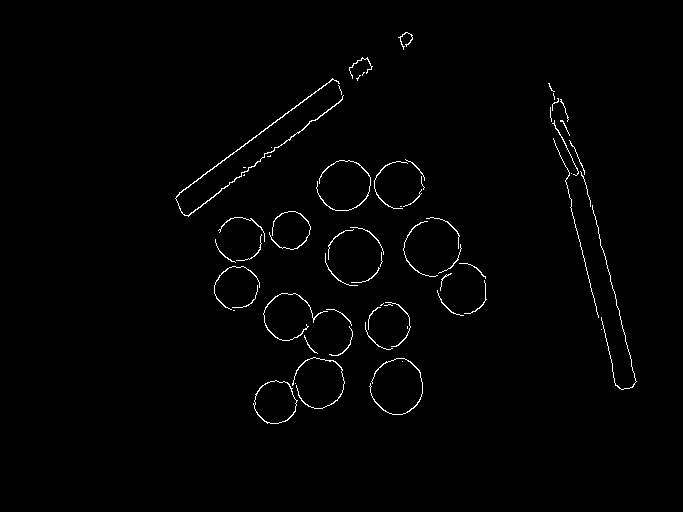
\includegraphics[width = .5\textwidth]{ps1-4-b-image-noisy-edges.png}
 \caption{ps1-4-b : Edges Smoothed Image }
\label{ps1-4-b}
\end{figure}

The Figure 7 shows the Canny edge detection result.

\subsection{Third Step : Hough Algorithm for lines}

 \begin{figure}[H]
\begin{center}
\begin{tabular}{cc}

\includegraphics[height = .5\textwidth]{ps1-4-c-accu-circled.png}&
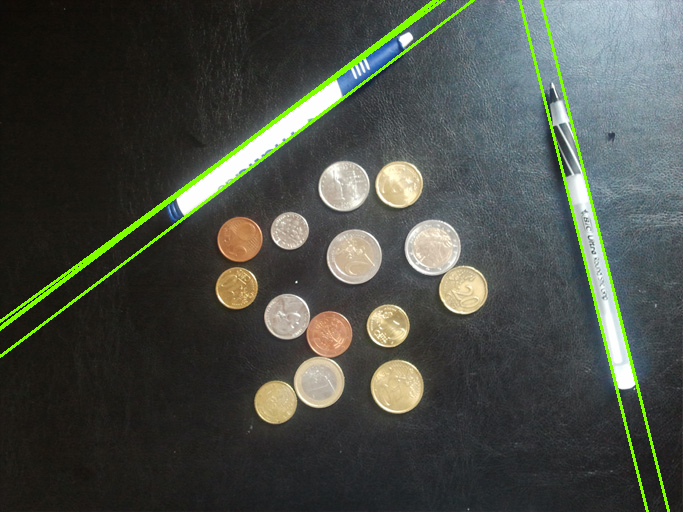
\includegraphics[height = .5\textwidth]{ps1-4-c-lines.png}\\
	a&b
\end{tabular}
\end{center}
 \caption{
\textit{a}. ps1-4-c-accumulator : Hough accumulator array image.  \textit{b}. ps1-4-c-lines : Intensity Image with lines drawn on them. }
\label{ps1-4-c}
\end{figure}

In order to get to the cleanly detected lines of the pens (Figure 8.b), we had to follow a similar process as previously.

This time we used a larger Gaussian kernel to get a wider extent of smoothing in order to avoid detecting any of the inner edges of the pens. The circles of the coins are less of a problem once we manage to keep them clean, since our Hough algorithm will target specifically the lines.

The resulting accumulator visible in Figure 8.a shows pair of peaks, corresponding to the parallel edges of the pens. We have twice the number of peaks as what is expected, since they are spaced of 180 degrees and result in superposing lines on the final image.

\section{Circles Detection}

 \begin{figure}[H]
\begin{center}
\begin{tabular}{cc}
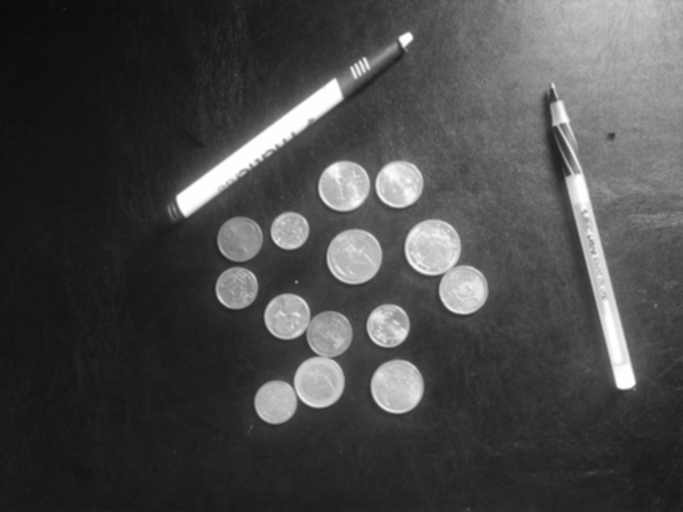
\includegraphics[width = .5\textwidth]{ps1-5-image-noisy-smoothed.png}&
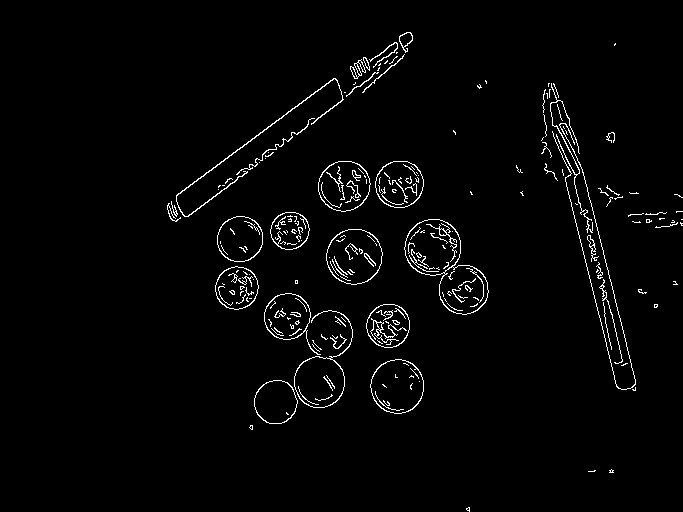
\includegraphics[width= .5\textwidth]{ps1-5-edges-image-noisy.png}\\
	a&b\\
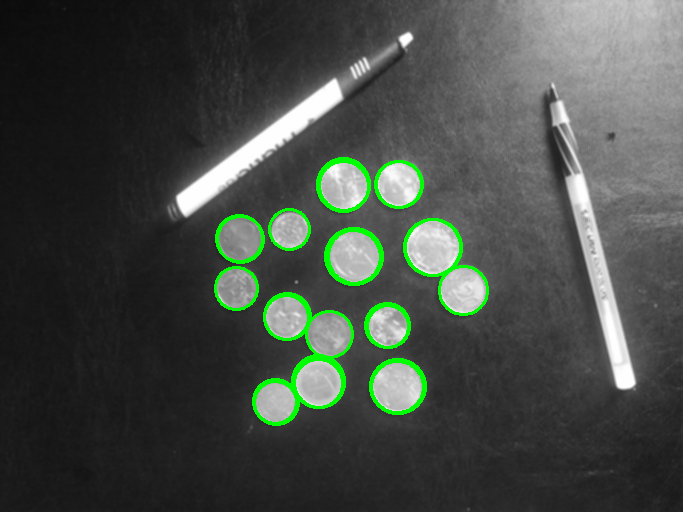
\includegraphics[width = .5\textwidth]{ps1-5-circles.png}\\
c
\end{tabular}
\end{center}
 \caption{
\textit{a}. ps1-5-smoothed : Image Noisy Smoothed.  \textit{b}. ps1-5-edges : Edges Smoothed Image.
\textit{c}. ps1-5-circles : Image with circles drawn in color. }
\label{ps1-5}
\end{figure}

Now our aim is to detect the coins on the image, we have to change the Hough transform to adapt it for circles meaning we have to take in account 3 parameters which are the cartesian coordinates of the circle center and the radius of the circle.

We first have to operate a light smoothing indeed it's not as important as in the previous question since the inner edges are not circular.
The Figure 9.b shows the result of the Canny edge detector.

We estimate the radius of the coins to be between 15 and 30 pixels, which is necessary in order to limit the computation time of our algorithm. 

For each edge point and each radius, we first computed the coordinates of the center for 180 values BUT in order to reduce the length of the computation an improvement of the algorithm was made by using the gradient to orient the search for a potential center.

Finally since the result gave some concentric circles superposed instead of a single, a "filtering" was made by taking into account the distance between the centers and by applying a threshold on it. A good solution seemed to take the mean circle for those really closed circles. We save then the radius and the center coordinate for that mean circle. It allows us to obtain the Figure 9.c. 


\section{Finding lines on a more realistic image}

\subsection{Application on a line finder}

The Figure 10.b is the result of the lines detection made by the Hough transform for lines after having tried to smoothe to put aside the edges of the text and barcode.

 \begin{figure}[H]
\begin{center}
\begin{tabular}{cc}
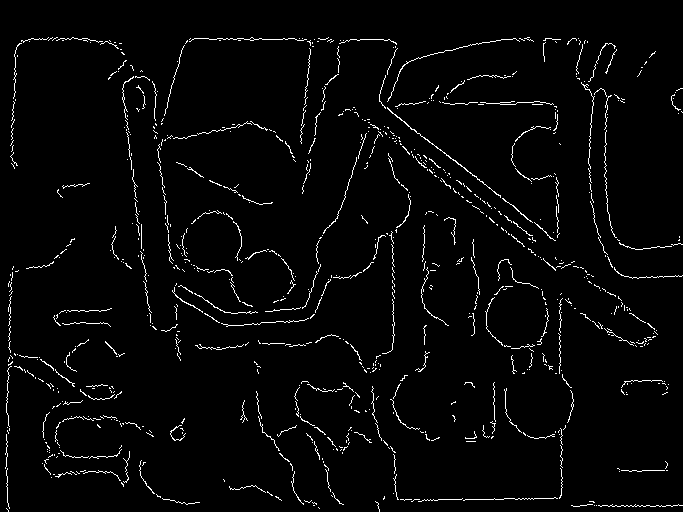
\includegraphics[width = .5\textwidth]{ps1-6-a-edges.png}&
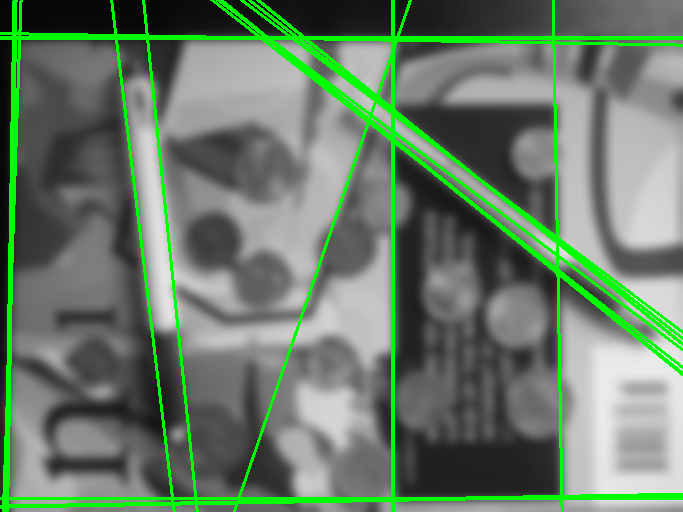
\includegraphics[width= .5\textwidth]{ps1-6-a-lines.png}\\
	a&b
\end{tabular}
\end{center}
 \caption{
\textit{a}. ps1-6-a-edges : Edges Image Smoothed.  \textit{b}. ps1-6-a-lines : Hough Lines drawn on the smoothed image.}
\label{ps1-6}
\end{figure}

\subsection{Problems with our line finder}

Many lines are rightfully detected by the algorithm because of the magazine cover borders and geometric content. 

Now since we want to focus on the boundaries of the pen, we will rely on the fact that those lines are parallel edges, space by a minimal distance, in order to filter out the undesirable edges.


\subsection{Attempt to find the boundaries lines of the pen}


Applying a maximum distance (to avoid the magazine cover borders which are parallels too), a minimum distance (to avoid the superposed lines)and specifying the maximum and minimum angle between two lines to be considered parallel, we manage to extract the pens boundaries as visible in Figure 11.

\begin{figure}[H]
\centering
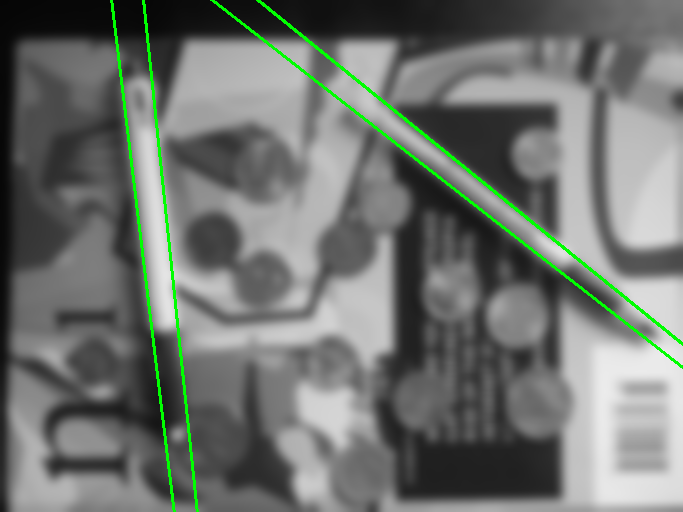
\includegraphics[width = .5\textwidth]{ps1-6-c-lines.png}
 \caption{ps1-6-c :New Hough lines drawn on the smoothed image}
\label{ps1-6-c}
\end{figure}

\section{Finding Circles on the same clutter image}


By applying the Hough circle transform on the cluttered image, we manage to detect some of the coins but not all. A tradeoff has to be made on the threshold. A lower threshold, even after having realized a really effective smoothing (as shown on Figure 12.b), was providing a lot of false alarms. Here this threshold avoids the false alarms but does not allow to obtain all the circles.
The result is presented on Figure 12.c.

 \begin{figure}[H]
\begin{center}
\begin{tabular}{cc}
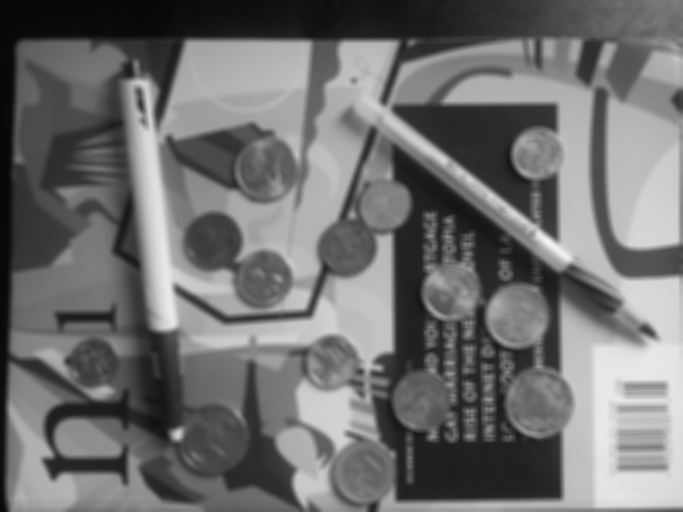
\includegraphics[width = .5\textwidth]{ps1-7-image-noisy-smoothed.png}&
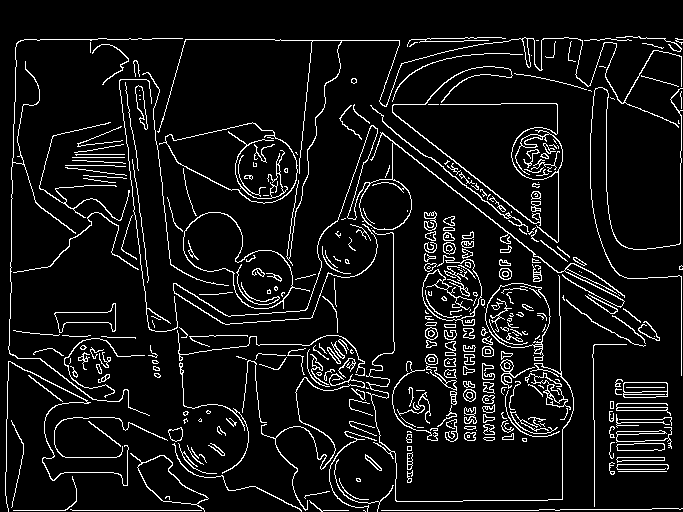
\includegraphics[width= .5\textwidth]{ps1-7-edges-image-noisy.png}\\
	a&b\\
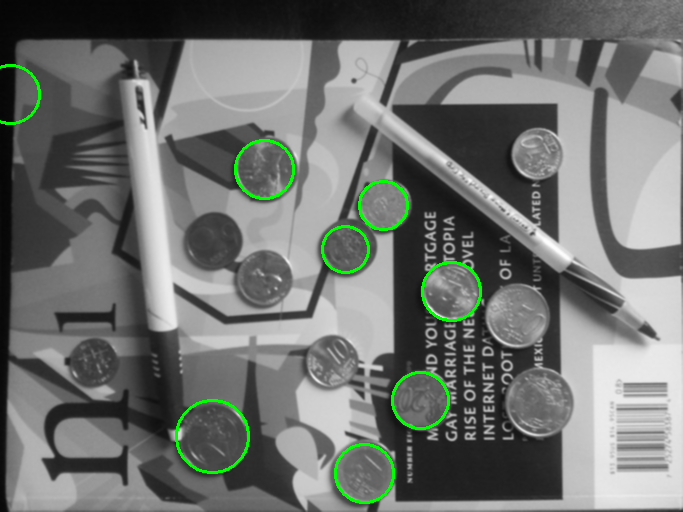
\includegraphics[width= .5\textwidth]{ps1-7-circles.png}\\	
\end{tabular}
\end{center}
 \caption{
\textit{a}. ps1-7-a-smoothed : Smoothed Image.  \textit{b}. ps1-7-a-edges : Edges Image Smoothed. 
\textit{c}. ps1-7-a-circles :  Hough Circles drawn on the smoothed image.}
\label{ps1-7}
\end{figure}

\section{Sensitivity to distortion}

\subsection{Application of the line and circles finder}

 \begin{figure}[H]
\begin{center}
\begin{tabular}{cc}
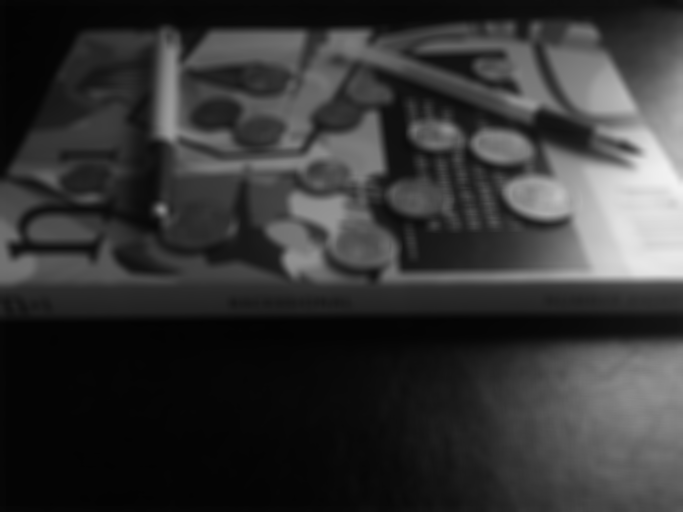
\includegraphics[width = .5\textwidth]{ps1-8-image-noisy-smoothed.png}&
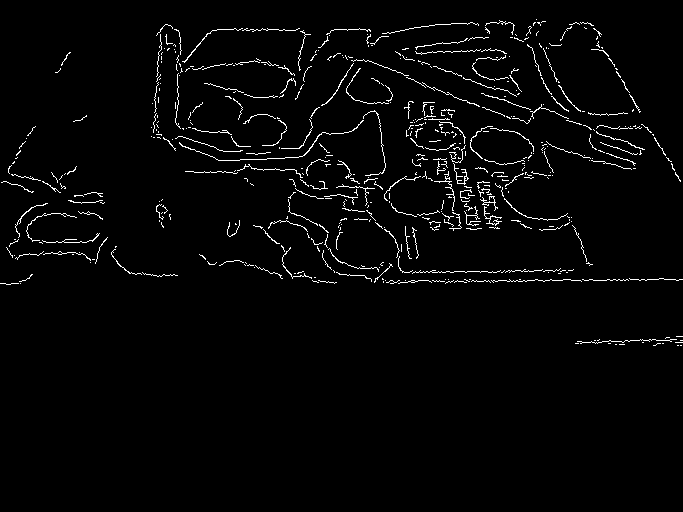
\includegraphics[width= .5\textwidth]{ps1-8-edges-image-noisy.png}\\
	a&b\\
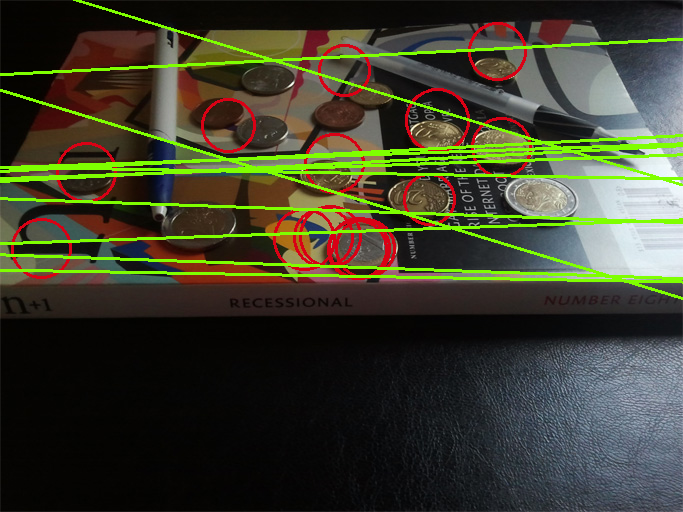
\includegraphics[width= .5\textwidth]{ps1-8-circles.png}\\	
\end{tabular}
\end{center}
 \caption{
\textit{a}. ps1-7-a-smoothed : Smoothed Image.  \textit{b}. ps1-7-a-edges : Edges Image Smoothed. 
\textit{c}. ps1-7-a-circles :  Hough Circles and Hough Lines drawn on the smoothed image.}
\label{ps1-7}
\end{figure}

Our two Hough transforms applied to a distorted image do not perform well (Figure 13.c). Even with a parallel lines filtering, which should help detect the pens even in this setup, we do not manage to extract any of their boundaries but still get unwanted edges.

However, the circles detection seems to perform slightly better, despite plenty of false alarms it seems that we detect several coins, as well as the false circle visible in the "n" letter.

\subsection{How to fix the problem ?}

Future enhancements of our code would be to adapt the circle transform to an ellipse one. Indeed with the distortion, the circles become ellipses.We would however probably face at least the same amount of false alarms as in the previous section, and would also need to implement further improvements.

Regarding the lines, we would need to adapt the smoothing and edge detection to also take into account the stronger impact of the shadows on this distorted version of the image. We could also add constraints on the filtered lines to look for lines at specific angles and with a specific number of close parallel edges.

\end{document}